\section{Einleitung}

Ziel dieser Arbeit ist die Untersuchung von Methoden zur automatisierten Bestimmung der Farbwerte von Oberflächenelementen in Webseiten, welche sich an einer Bildvorlage orientieren. Die Beantwortung dieser Fragestellung erfolgt durch den Vorschlag und die Umsetzung eines konkreten Verfahrens. \autoref{sec:modellierung} unternimmt eine grundlegende Modellierung des Färbungsproblems in Bezug auf Webseiten und legt  den Rahmen der Zielstellung fest. \autoref{sec:cpe} stellt das Teilproblem der Ermittlung repräsentativer Farben eines Bildes vor. \autoref{sec:literatur} ordnet die Arbeit in den aktuellen Forschungskontext ein.

\subsection{Problemmodellierung}
\label{sec:modellierung}

\begin{figure*}[h]
	\centering
	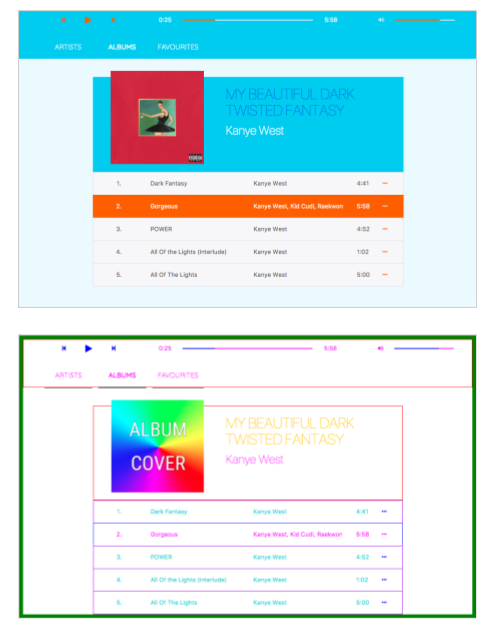
\includegraphics[width=1\textwidth]{img/color_groups.png}
	\caption{Beispiel der Farbgestaltung einer exemplarischen Weboberfläche für Musik-Streaming. (a) Generische Farbgestaltung ohne Anpassung an das Albumcover. (b) Separate Hervorhebung der sechs Color Groups. Elemente einer Color Groups sind jeweils rot dargestellt. (c) Beispiel einer Farbgestaltung mit Anpassung an das Album Cover.}
	\label{fig:colorgroups}
\end{figure*}

Der CSS-Standard zur Beschreibung der Formatierung von HTML-Dokumenten definiert mehr als 10 Eigenschaften zur farblichen Gestaltung, wobei einige spezifisch für bestimmte  HTML-Elemente sind  \citep{css3-color}. In dieser Arbeit werden die Farbeigenschaften von zwei verschiedenen Arten von Oberflächenelementen $e = (c_\text{text}, c_\text{background}) = C \times C$ betrachtet:
\begin{enumerate}
	\item \textbf{Textelemente} $e_\text{Text}$: Elemente mit transparentem Hintergrund und definierter Vordergrundfarbe (z.B. \texttt{<h1>}, \texttt{<a>}, etc.). Diese besitzen die CSS-Eigenschaften \{ \texttt{background-color: transparent}, \texttt{color:} $e.c_\text{text}$\}.\\ Dementsprechend gilt: $type(e) = \text{Text} \implies e.c_\text{background} = "\text{transparent}"$.\\
	\item  \textbf{Blockelement} $e_\text{Block}$: Elemente, die visuell als Blöcke wahrgenommen werden (z.B. \texttt{<div>}, \texttt{<button>}, etc.). Diese besitzen die CSS-Eigenschaften \{ \texttt{background-color:} $e.c_\text{background}$, \texttt{color:} $e.c_\text{text}$\}.
\end{enumerate}
Es wird also die Farbbestimmung von Vorder- und Hintergrundfarben fokussiert. Rahmen, Textdekoration und andere färbbare Eigenschaften werden vernachlässigt.

Üblicherweise werden mehrere Elemente eines HTML-Dokuments auf die gleiche Farbe abgebildet. Ein Beispiel ist die Darstellung aller Links ($e.c_\text{text}$) sowie Buttons ($e.c_\text{background}$) in Blau. Im Folgenden wird eine Liste von Elementen einer Webseite mit gleicher Farbabbildung als \textbf{Color Group} $CG = (e_1, e_2, ...) $ bezeichnet \citep[siehe auch][]{webpage, patterns}. Die Menge aller Color Groups einer Webseite heißt \textbf{Color Groups} $CGs = \{CG_1, ... CG_k\}$ mit $|CGs| = k$. Abbildung \ref{fig:colorgroups} veranschaulicht dies anhand einer exemplarischen Webseite für Musik-Streaming. (a) zeigt ein generisches Farbdesign, während (b) die sechs Color Groups separat hervorhebt.

\textcolor{red}{TODO: Abbildung updaten}

Webdesigner verkleinern den Suchraum zur Identifizierung geeigneter Farben für die Color Groups durch die Verwendung einer sogenannten \textbf{Farbpalette} \citep{webpage, webdesign, webx0}. Dabei handelt es sich um eine Farbmenge $P = \{c_1, c_2, \ldots, c_n\}$ mit $n$ Farben, wobei jedes $c \in P$ als String von RGB Werten kodiert wird. \textbf{Die Farbgestaltung einer Webseite ist die Abbildung $f_\text{coloration}: CGs \to P$} mit folgender Definition:

\begin{equation}
\begin{gathered}
  f_\text{coloration}: CGs \to P,\; \\[-1mm] 
  \mathclap{\rule{4cm}{0.4pt}}\\
  f_\text{coloration}(CG) = c \implies \forall e \in CG:
  	\begin{cases}
		e.c_\text{text} = c, \; \text{wenn } type(e) = \text{Text} \\
		e.c_\text{background} = c, \; \text{wenn } type(e) = \text{Block}
	\end{cases}
\end{gathered}
\end{equation}

Entscheidendes Kriterium für die Zuordnung  ist eine funktionale Gestaltung der Webseite. Im Rahmen dieser Arbeit wird hierunter eine Färbung der Oberflächenelemente verstanden, die \textbf{Textlesbarkeit} und \textbf{Benutzerführung} gewährleistet. Eine intuitiv widersinnige Färbung ist beispielsweise roter Text auf orangem Hintergrund mit grauem Button. Weder ist der Text lesbar, noch wird die Aufmerksamkeit des Nutzers auf das Interaktionselement gelenkt.

Die Farbpalette soll auf einer Bildvorlage basieren. So wird eine Harmonisierung des visuellen Eindrucks einer Weboberfläche und einer darin präsenten Grafik erreicht. Da die Farben einer Webseite wesentlich für deren vermittelte Atmosphäre sind \citep{webdesign}, soll die Anpassung der Farbgebung an ein Motiv den Eindruck des Bildes unterstützen. Da die Farbpalette somit auf den verarbeiteten Daten basiert, ist eine Berechnung der Farbgestaltung einer Webseite zur Laufzeit möglich. Ein Anwendungsbeispiel hierfür ist die farbliche Anpassung einer Webanwendung für Musikstreaming an das gespielte Albumcover. Abbildung \ref{fig:colorgroups} (c) zeigt hierfür ein Beispiel. Die Ermittlung von $P$ aus einer Grafik wird als Color Palette Estimation bezeichnet und im Folgenden besprochen.

\subsection{Color Palette Estimation}
\label{sec:cpe}

Die Abbildung einer Bildvorlage $I$ auf eine Farbpalette $P$ wird von \citet{acopa} als \textbf{Color Palette Estimation} (CPE) $f_{CPE}: I \to P$, bezeichnet und als die Repräsentation eines Bildes mit einer minimalen Menge von Farben beschrieben. \glqq{}Minimal\grqq{} bedeutet nach Auffassung der Autoren, dass redundante Farben reduziert und die seltenen Farben der für die Wahrnehmung wichtigen Objekte erhalten bleiben. Formale Kriterien werden hierfür jedoch nicht geliefert. Abbildung \ref{fig:ladybug} veranschaulicht diese intuitive Definition am Beispiel eines Bildes mit einem Marienkäfer, dessen Sichtbarkeit von der Wahl der Farbpalette abhängt.

\begin{figure}[h]
\centering
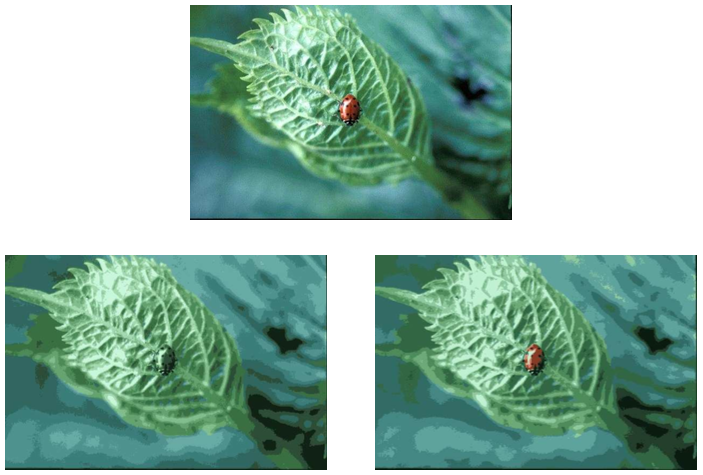
\includegraphics[width=0.5\textwidth]{img/ladybug.png}
\caption{Beispiel für die Einfärbung eines Bildes mit unterschiedlichen Farbpaletten der Größe 12. Oben: Originalbild. Links: Farbpalette ohne rote Farbtöne. Rechts: Farbpalette mit roten Farbtönen, wodurch der Marienkäfer erkennbar ist (Quelle: \citep{acopa})}
\label{fig:ladybug}
\end{figure}

Historisch geht die CPE aus der Farbquantisierung hervor, bei der die Farben von Grafiken aufgrund der damals zu kleinen Kapazität von Grafikpuffern vor deren Anzeige reduziert (Farbreduktion) und dann auf die reduzierte Farbpalette abgebildet wurden (Quantisierung) \citep{variance}. Aus diesem Kontext kommt das formale Kriterium der Summe des quadratischen Fehlers, welcher in diesem Anwendungsfall auch als \emph{Recoloring Error} bezeichnet wird \citep{colorthemes}. Da Grafikpuffer mittlerweile über ausreichend Kapazität verfügen liegt die Anwendung der CPE in anderen Bereichen, wie z.B. der farbbasierten Indizierung von Grafiken in Datenbanken oder der Zusammenstellung von Farbpalletten zu Gestaltungszwecken. \citet{colorthemes} zeigen, dass in letzterem Kontext der Recoloring Error keine geeignete Metrik zur Beurteilung der Güte einer Farbpalette in Bezug auf die Bildvorlage ist. Dies beruht auf den menschlichen Wahrnehmungseigenschaften, wobei Bilder auf Komponenten- und nicht auf Pixelebene erfasst werden. Stattdessen werden eine Reihe anderer Metriken vorgestellt, die diesen Umstand berücksichtigen. Die Autoren zeigen zusätzlich empirisch, dass abhängig vom Individuum ein und dieselbe Farbpalette im Bezug auf die Bildvorlage als unterschiedlich repräsentativ bewertet wird.

Dieser Befund hebt hervor, dass die Güte der Abbildung $I \to P$ subjektiv ist und vom Anwendungsbezug abhängt. Aus diesem Grund wird für die Beurteilung der zu ermittelnden Farbpalette keine objektive Bewertungsfunktion herangezogen. Stattdessen wird die Auswahl eines Algorithmus zur CPE fokussiert, dessen resultierende Farbpalette zweckmäßig in Hinblick auf die farbliche Gestaltung von Webseiten ist. Hierfür werden in \autoref{sec:farbgestaltung} Prinzipien für eine funktionale Gestaltung von Webseiten sowie Farbdefinitionen in Style Guides analysiert.

\subsection{Einordnung und Literaturbesprechung}
\label{sec:literatur}

Diese Arbeit ordnet sich in das Gebiet der automatisierten Farbgestaltung (\emph{Color Design Automation}) ein. In diesem Bereich hat in den letzten Jahren Forschung in verschiedenen Anwendungsbezügen stattgefunden, wobei überwiegend Methoden des maschinellen Lernens zur Problemlösung zum Einsatz kommen.

\citet{colorcomp} haben 2011 ein Regressionmodell zur Bewertung der Farbkompatibilität von bis zu fünf Farben entwickelt, d.h. zur Bewertung der Farbharmonie einer Farbpalette. Hierfür wurde ein Training an den Datenbeständen von Farbpaletten-Communities wie z.B. Adobe Color\footnote{\url{https://color.adobe.com/de/explore/}} durchgeführt. Dabei hat sich unter anderem ergeben, dass die auf geometrischen Strukturen im Farbkreis beruhenden Modelle der klassischen Farbentheorie Farbhamonien nicht zufriedenstellend voraussagen und in bestimmten Fällen sogar kontraproduktiv sind. Hierzu zählen zum Beispiel die Farbton-Schablonen von \citet{itten} oder \citet{munsell}. Die Grenzen des Modells liegen in der Bewertung der Harmonie von Farben mit unterschiedlicher räumlicher Ausprägung \citep{webpage, patterns}. Eine Matlab-Implementierung des Modells zur Überprüfung von Farbharmonien steht öffentlich zum Download bereit\footnote{\url{http://www.dgp.toronto.edu/~donovan/color/}}.

\citet{patterns} haben sich 2013 mit der Lösung einer grundlegenden Form eines Färbungsproblems auseinandergesetzt: Die Kolorierung von Mustern nach dem Prinzip "Malen nach Zahlen". Hierfür wurde ein probabilistisches Modell entwickelt, indem über 8000 von Künstlern entworfene Muster ausgewertet wurden\footnote{\url{http://www.colourlovers.com/}}. Konkrete Färbungslösungen werden durch einen \emph{Factor Graph} ermittelt, was ebenfalls einen Ansatz für die vorliegende Arbeit darstellt. Das Modell von \citet{colorcomp} wird als externer Bestandteil des Graphen hinzugefügt, um eine globale Kompatibilität der eingesetzten Farben zu gewährleisten. Eine Anwendung, welche die Autoren vorschlagen, stellt die Umkehrung des Ziels dieser Arbeit dar: Die Anpassung eines Musters an das Farbschema einer Webseite.

\citet{webpage} haben sich 2016 mit der automatisierten Farbgestaltung von Webseiten auseinandergesetzt. Durch die Auswertung von 500 Webseiten wurde ein probabilistisches Modell in Form eines Optimierungsproblem mit drei Zielfunktionen entwickelt. Zielfunktionen 1 gewährleistet einen ausreichenden Kontrast zwischen den Oberflächenelementen. Zielfunktion 2 passt die Farbgestaltung an ein Schlüsselwort an (z.B. \glqq{}Business\grqq{} oder \glqq{}Fresh\grqq{}). Zielfunktion 3 wird durch das Modell von \citet{colorcomp} realisiert und gewährleistet Farbharmonie. Die Optimierung wird durch eine lexikographische Strategie umgesetzt, bei welcher in Interaktion mit einem Gestalter die Zielfunktionen nacheinander angewendet werden. Die Farben zur Seitenfärbung werden Farbpaletten von Adobe Color\footnote{\url{https://color.adobe.com/de/explore/}} entnommen. Als alternatives Anwendungsbeispiel extrahieren die Autoren eine Farbpalette aus einer Grafik und nutzen diese als Grundlage zur Färbung, was dem Ziel der vorliegenden Arbeit entspricht. Zur CPE wird der K-Means Algorithmus verwendet. Somit ist der vorgestellte Prozess der Autoren im Gegensatz zum Ziel dieser Arbeit lediglich teilautomatisiert. Einerseits muss ein geeignetes $k$ des K-Means Algorithmus vom Anwender ermittelt werden, andererseits erfordert die lexikographischen Strategie bei der Optimierung eine Nutzerinteraktion. Somit handelt es sich bei der Lösung um ein Unterstützungswerkzeug für Webdesigner und nicht um ein System zur vollautomatisierten Farbgestaltung einer Webseite.

\citet{magazines}  haben sich 2013 mit der automatisierten Farbgestaltung von Magazin-Covers auseinandergesetzt. Vergleichbar mit \citep{webpage} wird ebenfalls die Optimierung des Farbkontrasts, der Farbharmonie und der Farbsemantik verfolgt. Im Gegensatz zu den bisherigen Lösungen wird allerdings mit expliziten Regeln zur Bewertung von Farbharmonien- \citep{itten} und Kontrasten anstatt mit Modellen gearbeitet, die sich aus Trainingsdaten ableiten. Über Flowcharts vermitteln die Autoren Lösungsprozeduren zur Suche geeigneter Schriftfarben unter Beachtung des Kontrasts, welche eine Anregung für die vorliegende Arbeit darstellen.